\documentclass[10pt,onecolumn,twoside,letterpaper]{article}
\usepackage[text={7in,9.5in},centering]{geometry}
\usepackage[spanish,es-nodecimaldot]{babel}

\usepackage{hyperref}

\usepackage{multicol}

\usepackage{harvard}% bibliographystyle: apsr, agsm, dcu, kluwer, nederlands

\usepackage{graphicx}
\usepackage{amssymb}
\usepackage{fancyhdr}
\usepackage{color}
\usepackage{colortbl}
\definecolor{gray}{cmyk}{0.0,0.0,0.0,0.60}

%\usepackage{auto-pst-pdf}
%\usepackage{pst-all}

%\usepackage[numbered]{mcode}
%\usepackage{lipsum}

\pagestyle{fancy}
\fancyhf{}
\fancyhead[RO]{\small{\textcolor{gray}{\textsc{Hacia un framework de locomoci\'on b\'ipeda evolutiva y flexible}}}}
\fancyhead[LO]{
\includegraphics[scale=0.05]{../../images/unlogo.png}}
\fancyhead[LE]{
\includegraphics[scale=0.05]{../../images/unlogo.png}\quad\small{\textcolor{gray}{\textsc{Linea de investigaci\'on: Robotica Evolutiva en Caminadores}}}}
\fancyfoot[CO,CE]{\thepage}
\fancyfoot[LO,RE]{\scriptsize{\textcolor{gray}{\emph{Version 0.2}}}}

\title{\vspace{-0.8cm}
\includegraphics[scale=0.12]{../../images/unescudobn.png}\\\vspace{-0.0cm}
  \LARGE \textbf{Robots saltarines y direcci\'on dirigida por objetivos}}
\author{J.A. Castillo-Le\'on\thanks{jacastillol@unal.edu.co} \and R.E. Ram\'irez-Heredia\thanks{reramirezh@unal.edu.co}}
\date{}

\begin{document}
\maketitle
\begin{abstract}\small
  Este trabajo esta enfocado a la construcci\'on de un prototipo de bajo costo de un robot viga-saltarin. Se requiere fundamentos de dise\~no, fundamentos b\'asicos de FEM, programaci\'on en MATLAB y conocimientos de electr\'onica.
\end{abstract}
%\begin{multicols}{2}
\section{Descripci\'on:}
Explorando la relaci\'on de las resonancias de la estructura y los distitos patrones de movimiento, se puede controlar la direcci\'on de movimiento con tan solo variar la frecuencia de rotaci\'on del motor\cite{Reis2014}.
\section{Objetivo:}
El objetivo principal es contruir un robot viga-saltar\'in con masa de rotaci\'on decentrada de la base y proponer un control b\'asico de movimiento de la estructura con solo la variacion de la variacion de la velocidad del motor. Se necesita contrastar los resultados con un modelo te\'orico en FEM de un modelo din\'amico. Se entraga modelo simple en FEM en MATLAB.
%\end{multicols}
\begin{figure}[!ht]
  \centering
  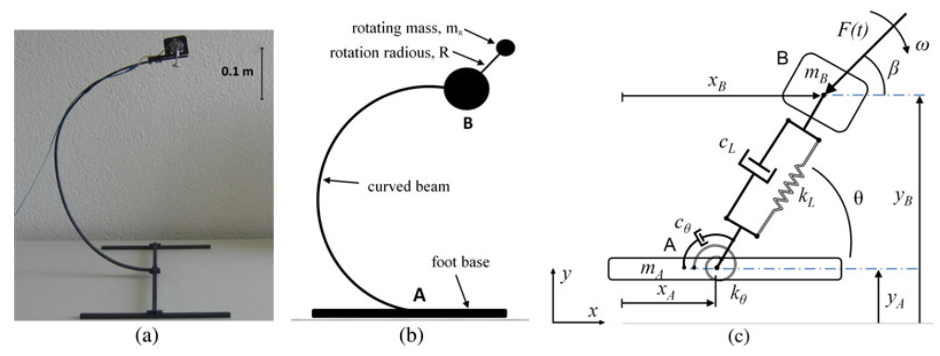
\includegraphics[scale=0.4]{../../images/ReisBeamModelRobot.png}
  \caption{Modelo D\'namico General}
  \label{fig:grizmodelo}
\end{figure}
%\nocite{*}
\bibliographystyle{nederlands}% apsr, agsm, dcu, kluwer, nederlands
\bibliography{../../review/review/library}
\end{document}
